% DOCUMENT
%\documentclass[a4paper]{article}
\documentclass[a4paper, twocolumn]{article}

% PACKAGES
\usepackage{titlesec}
\usepackage[english]{babel}
\usepackage{blindtext}
\usepackage{graphicx} 
\usepackage{enumitem}
\usepackage{amsmath}
% \usepackage{parskip}
\usepackage{mathptmx}
% \usepackage[none]{hyphenat}
%\usepackage[showframe]{geometry}
\usepackage{layout}
\usepackage[bottom=0.5in]{geometry}
\usepackage{float}

% SETTINGS
% Title Format
\titleformat*{\section}{\large\bfseries\MakeUppercase}
\titleformat*{\subsection}{\large\MakeUppercase}
\titleformat*{\subsubsection}{\large}

% USER-DEFINED COMMANDS

% TITLE
\title{\Huge{MPC based Path Tracking using Potential Field for Autonomous Mobile Robot}}
\author{Faizudeen Olanrewaju Kajogbola} 
% \affiliation{Technische Universität Kaiserslautern}
\date{} %BLANK DATE TO OMIT DATE FROM TITLE

% DOCUMENT
\begin{document}

% DISPLAY TITLE
\maketitle

\setlength{\headsep}{5pt}
\setlength{\voffset}{-0.75in}   % REMOVE EXCESSIVE SPACE AT TOP OF PAGE

% INTRODUCTION
\section{Introduction}

Autonomous Mobile Robots (AMRs) are required to move around to perform some tasks, 
this makes the ability to navigate effectively and efficiently an important measure of success for any such robot.
For navigation, an AMR is required to plan a path leading to its goal point, 
generate a trajectory along the planned path, and appropriately track such generated trajectory.

Path planning involves searching for an optimal collision-free path from an initial position to some 
desired goal position which conforms to its physical constraints of the AMR in question \cite{cai1}.
Path planning is divided into: global path planning in which the environment known completely; 
and the local path planning in which only some section of the environment is known.
Common global path planning techniques include A* heuristic search, visibility graph method, generalized Voronoi diagram, 
ant colony algorithm, genetic algorithm, and the artificial potential field method \cite{kunchev1, shi1}.

The Artificial Potential Field (APF) method draws inspiration from classical physics and was first proposed in 1986 by Khatib \cite{khatib1}.
With this method, an AMR seems to move towards its goal position and avoid obstacles instinctively. 
This is because repulsive potentials are generated to represent obstacles, while attractive potentials are 
generated to represent the goal position, effectively transforming the path planning problem into an 
optimization problem \cite{ji1}. 

APF approach gives room for the possibility of real-time online path planning. 
Globally planned paths can be updated with local information from robot sensors- 
e.g. new location of a moving obstacle, thereby making it possible to plan paths that avoid dynamic obstacles.
This, and its mathematical conciseness \cite{shi1} are some of the reasons why APF-based approaches 
are widely used in path planning for AMRs.
However, if special care is not taken in formulating the potential functions, the robot might get stuck at 
a local minimum and thereby never reaching its goal position.
To prevent this, several methods of formulating the potential functions have been proposed. 
These include gaussian-shaped repulsive functions \cite{koditschek1}, the super-quadratic potential function \cite{volpe1}, 
simulated annealing technique \cite{zhu1}, and methods that utilize search techniques with the capability of escaping local minima \cite{barraquand1}.

A trajectory can be generated from a planned path by time parametrization \cite{roesmann1}. 
To enable collision-free navigation, the generated trajectory must respect the dynamical and kinematical constraints of the AMR.
Due to nonlinear dynamics, path tracking of AMRs is generally performed using sliding mode control \cite{yang1}, 
robust control \cite{normey-rico1}, fuzzy logic control \cite{antonelli1}, or model predictive control (MPC) \cite{ji1}.

In recent years, a lot of research efforts have been poured into implementing MPC algorithms for navigation.
Götte et al. in \cite{goette1} propose a model predictive planning and control (MPPC) approach which handles both trajectory planning and tracking.
In \cite{nolte1}, Nolte et al. present a generalized approach for path and trajectory planning with model predictive frameworks.
A constrained linear time-varying MPC was implemented by Gutjahr et al. in \cite{gutjahr1} for path tracking and trajectory optimization.
While a multi-constrained MPC was presented by Ji et al. in \cite{ji1} solely for the purpose of path-tracking.

In the following, path tracking and obstacle avoidance for an AMR is investigated.
Avoidance of static obstacles in a completely known environment is considered, while taking the robot’s kinematic limitations 
(such as its size, shape, and its steering constraints) into account.
An APF approach is used for path planning and trajectory generation, 
while a multi-constrained model predictive control is used for tracking the generated trajectory. 
Two MPC controllers are designed, one based on a SISO system model, and the other based on a SIMO model. 
The performance of the two controllers along with a PID controller are compared under multiple simulation scenarios.


%===============================================================================================================%
\section{Path Planning and Trajectory Generation}
This section focuses on path planning and trajectory generation based on Artificial Potential Fields (APFs).
While many researchers have proposed a vast array of path planning techniques, APFs provide an intuitive formulation that 
allow real-time modifications of planned trajectories. A feature that becomes quite essential in configuration spaces with dynamic obstacles.

The following assumptions are made in this study to simplify the mathematical representation of collision-free trajectories:
\begin{itemize}[itemsep=2pt]
    \item A configuration space of 50m x 50m.
    \item Static obstacles with rounded geometry of known sizes and positions.
    \item Constant longitudinal velocity of 1m/s.
\end{itemize}

\subsection{Path Planning}
Two coordinate systems are considered. The Autonomous Mobile Robot's (AMR's) body coordinate system $\mathit{o-xy}$, 
which is centered on the vehicle's center of mass with the x-axis is along the AMR's longitudinal axis, 
while the y-axis is along it's lateral axis; and a fixed earth coordinate system $\mathit{O-XY}$, 
which is defined to be colinear with the vehicle body coordinate system at the instant of path planning. 
At any point in time, the angle of rotation between both coordinate systems is the AMR's yaw angle $\psi$. 
The position of the AMR in the fixed-earth coordinate is given as $\vec{X_{r}}$, 
the position of the goal point as $\vec{X_{g}}$, and position of obstacles as $\vec{X_{o}}$.

The universal potential ($U$) which guides the AMR to it's goal position is composed of the attractive potential ($U_{A}$) 
and the repulsive potential ($U_{R}$).

The attractive potential ($U_{A}$) is formulated such that it's minimum point is at the goal position. 
A mathematical expression for the attractive potential is given as:
$$
U_{A}(\vec{X_{r}}, \vec{X_{g}}):= \frac{1}{2} K_{att} {\begin{Vmatrix}\vec{X_{r}} - \vec{X_{g}}\end{Vmatrix}}^{2}
$$
\noindent
where \\
$K_{att}$ is a constant.

\noindent
An attractive potential field with AMR initial position $(0, 0)$ and 
goal position $(50, 30)$ and $K_{att}= 0.01$ is shown in Figure \ref{fig:u_att}.

\begin{figure}
    \centering
    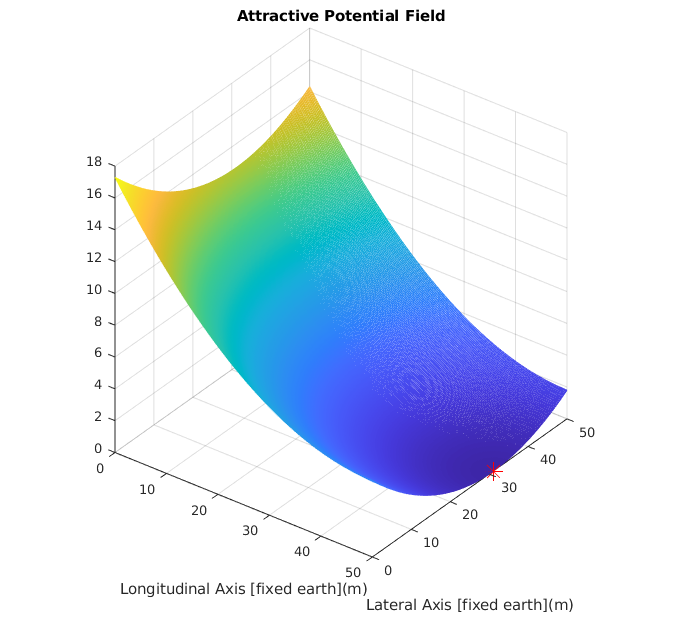
\includegraphics[scale=0.45]{presentation/img/u_att.png}
    \caption{Attractive Potential Field}
    \label{fig:u_att}
\end{figure}


The second component of the universal potential is the repulsive potential which results from superimposing 
the repulsive potential of each obstacle. The repulsive potential of an obstacle has it's peak at the obstacle's position and reduces as the 
distance from the obstacle increases. It can be expressed as: 



$$
    U_{R}(\vec{X_{r}}, \vec{X_{o}}):= 
    \begin{cases}
        \frac{1}{2} K_{rep} {\left( \frac{1}{\rho} 
        - \frac{1}{\rho_{0}} \right)}^{2}; &   \text{if}\ \rho < \rho_{0} \\

        0; & \text{otherwise} 
    \end{cases}
$$

\noindent
where \\
$\rho := \begin{Vmatrix}\vec{X_{r}} - \vec{X_{o}}\end{Vmatrix}$; \\
$K_{rep}$ is a constant; \\
$\rho_{0}$ is a constant that dictates the maximum distance from which the influence of an obstacle can be felt.
\noindent
A suitable selection according to kinetic theory is $\rho_{0} \geq V_{MAX}/2 A_{MAX}$ where $V_{MAX}$ is the 
maximum speed of the AMR and $A_{MAX}$ is the maximum deceleration of the AMR \cite{rostami1}.\\

Figure \ref{fig:u_uni_plot} shows the universal potential obtained by fusing the attractive potential from Figure \ref{fig:u_att} with repulsive 
potentials obtained from circular obstacles of radius $1m$ at coordinates (14.87, 33.28), (10, 8), (26, 12), (19, 19), and (34, 23) 
with $K_{rep}= 10$.


\begin{figure}
    \centering
    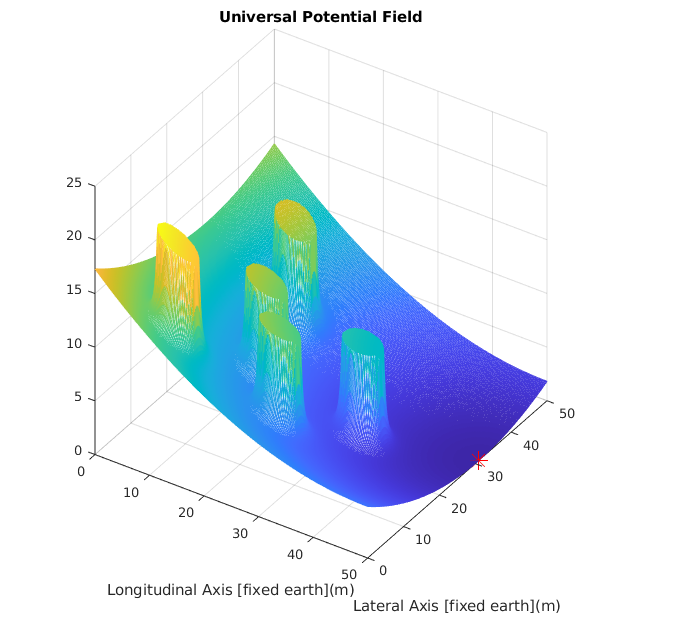
\includegraphics[scale=0.45]{presentation/img/u_uni_plot.png}
    \caption{Universal Potential Field}
    \label{fig:u_uni_plot}
\end{figure}


After setting up the universal potential, a simple gradient descent along this potential yields a "force" that guides the AMR towards the goal position 
while deflecting it away from the obstacles. This force can be interpreted as the velocity vector of the AMR along the planned path, 
and can be expressed as: 

$$F:= F_{A} + F_{R}$$

\noindent
where $F_{A}$ is the attractive force which is given by:
$$F_{A}(\vec{X_{r}}, \vec{X_{o}}):= -grad(U_{A})$$
$$F_{A}(\vec{X_{r}}, \vec{X_{o}})= -K_{att} \left(\vec{X_{r}} - \vec{X_{g}}\right)$$
\noindent
and $F_{R}$ is the repulsive force which is given by:
$$F_{R}(\vec{X_{r}}, \vec{X_{o}}):= \sum_{ \vec{X_{o}} \in \Omega}{-grad(U_{R})} $$
$$-grad(U_{R})= \frac{K_{rep}}{\rho^{3}} 
        \left( \frac{1}{\rho} - \frac{1}{\rho_{0}} \right) 
        \left(\vec{X_{r}} - \vec{X_{o}}\right) $$
\noindent
where 
$\rho= \begin{Vmatrix}\vec{X_{r}} - \vec{X_{o}}\end{Vmatrix}$; \\
$\Omega$ is a set of all obstacle coordinates.
 
Building upon the universal potential depicted in Figure \ref{fig:u_uni_plot}, 
Figure \ref{fig:path} shows the resulting collision-free path from the AMR's initial position (0, 0) to a goal position of (50, 30).

\begin{figure}
    \centering
    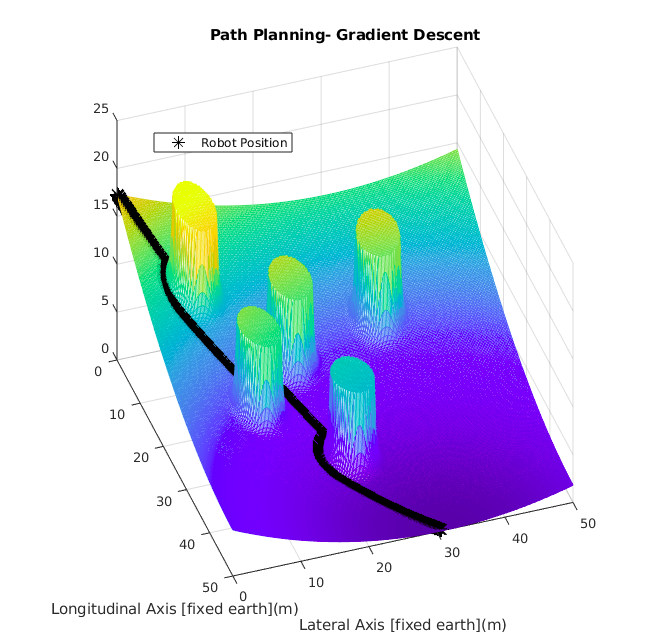
\includegraphics[scale=1.2]{presentation/img/path.png}
    \caption{Gradient descent along Universal Potential Field}
    \label{fig:path}
\end{figure}


\subsection{Trajectory Generation}

A planned path can be transformed into a trajectory by time-parametrizing it \cite{roesmann1}. 
Following from our earlier assumption of the AMR having a constant velocity of $1m/s$, 
we can generate a trajectory from our planned path by simulating forward in time along the planned path with a velocity 
vector of magnitude $1m/s$.

\begin{figure}[H]
    \centering
    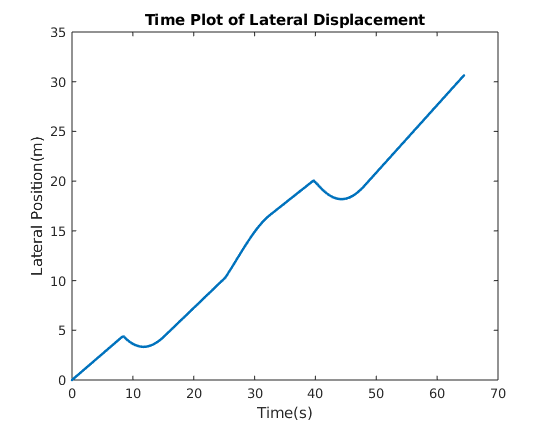
\includegraphics[scale=.45]{presentation/img/traj_lat.png}
    \caption{Trajectory Generation- Lateral Displacement}
    \label{fig:traj_lat}
\end{figure}

Figures \ref{fig:traj_lat} and \ref{fig:traj_lon} show the trajectory information for the path illustrated in Figure \ref{fig:path} simulated with a 
sampling time of 0.1 seconds.

\begin{figure}
    \centering
    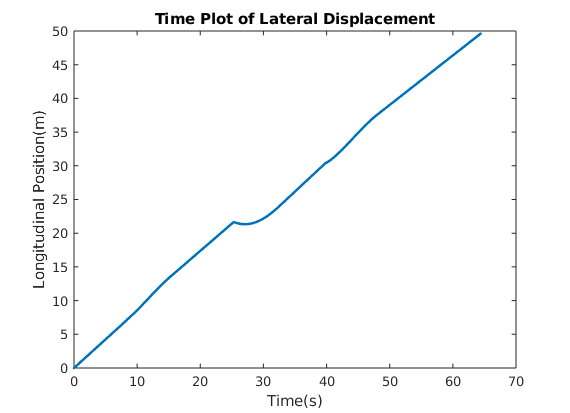
\includegraphics[scale=.45]{presentation/img/traj_lon.png}
    \caption{Trajectory Generation- Longitudinal Displacement}
    \label{fig:traj_lon}
\end{figure}

%===============================================================================================================%
% Mathematical Model
\section{Mathematical Model for Path Tracking Problem}

The mathematical model used for MPC design is described in this section. Since the success of any controller design is highly 
dependent on the accuracy of the plant model employed, correct modelling of the AMR is necessary. While the dynamics of 
AMRs are generally nonlinear, MPC allows us to base our design on a linearized model and still get satisfactory results. \\
For the path tracking problem considered in this paper, the following simplifying assumptions are made:
\begin{itemize}[itemsep=2pt]
    \item The AMR is a front wheel controller vehicle with a single front wheel and two rear wheels.
    \item Motion is only in the X-Y plane, i.e. rolling and pitching motions are ignored.
    \item Model parameters are constant.
    \item The AMR is operating in an indoor environment with a smooth and flat surface, such that gravitational and aerodynamic side forces can be ignored.
    \item Constant longitudinal velocity with perfect tracking along the longitudinal axis.
\end{itemize}

\begin{figure}
    \centering
    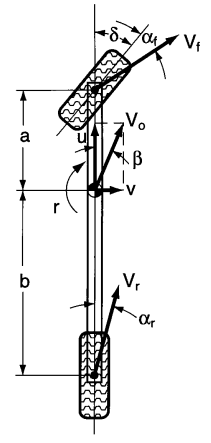
\includegraphics[scale=.45]{presentation/img/2DOF-bicycle.png}
    \caption{2 DOF Bicycle Model \cite{kiefer1}}
    \label{fig:2dof}
\end{figure}

\subsection{Dynamical Model for Lateral Path Tracking}
With the above assumptions, and also by lumping the two rear wheel into a single wheel, the linear two degree of freedom bicycle model (shown in FIgure \ref{fig:2dof}) of a 
conventional vehicle can be employed.

\noindent
Considering Newton's law of conservation of momentum along the lateral-axis, we have:

$$
F_{xf}cos(\delta) + F_{xr}= m(\dot{u} - \dot{\psi}v)
$$
$$
aF_{xf}cos(\delta) - bF_{xr}= I_{zz}\dot{r}
$$
\\
\noindent
Front tyre slip angle
$$
\gamma_{f}= atan\left(\frac{u+a\dot{\psi}}{v}\right)- \delta
$$
Rear tyre slip angle
$$
\gamma_{r}= atan\left(\frac{u-b\dot{\psi}}{v}\right)
$$

\noindent
Front tyre lateral force
$$
F_{xf}= C_{f}\gamma_{f}
$$
\noindent
Rear tyre lateral force
$$
F_{xr}= 2C_{r}\gamma_{r}
$$

\noindent
Sideslip angle
$$\beta= atan\left(\frac{u}{v}\right)$$
\\

\noindent
With small angles approximations, the sideslip angle can be approximated as 
$$\beta= \frac{u}{v}$$
\noindent
The front tyre angle as
$$\gamma_{f}= \frac{u+a\dot{\psi}}{v}- \delta= \beta + \frac{a\dot{\psi}}{v}+ \delta$$
\noindent
And the rear tyre angle as
$$\gamma_{r}= \frac{u-b\dot{\psi}}{v}= \beta- \frac{b\dot{\psi}}{v}$$


\noindent
The equations of motion then yield the following differential equations:

\footnotesize 
$$
\dot{\beta}= -\frac{\beta}{mv}\left( C_{f} + 2C_{f} \right) + r \left[\frac{1}{mv^{2}} \left(2bC_{r} 
    - aC_{f}\right)\right] + \delta \frac{C_{f}}{mv}  
$$

$$
\dot{r}= -\frac{\beta}{I_{zz}}\left(aC_{f} - 2bC_{r}\right) - r \left[\frac{1}{I_{zz}v} 
    \left(a^{2}C_{f} + 2b^{2}C_{r}\right) \right] + \delta \frac{aC_{f}}{I_{zz}} 
$$
\\

\normalsize
\noindent
By selecting the state variables:
\begin{itemize}[itemsep=2pt]
    \item Lateral displacement of CoM, $x_{c}$
    \item Side-slip angle, $\beta$
    \item Yaw angle, $\psi$
    \item Yaw velocity, $r$
\end{itemize}

\noindent
The following state space representation of the system is obtained
\footnotesize
$$
\begin{bmatrix}
    \dot{x_{c}}
    \\
    \dot{\beta}
    \\
    \dot{\psi}
    \\  
    \dot{r}
\end{bmatrix}=
\begin{bmatrix}
    0 & v & v & 0 \\ 
    0 & -\frac{C_{f}+2C_{r}}{mv} & 0 & \frac{2bC_{r} - aC_{f}}{mv^{2}} -1 \\ 
    0 & 0 & 0 & 1 \\ 
    0 & \frac{2bC_{r} - aC_{f}}{I_{zz}} & 0 & -\frac{\left(2b^{2}C_{r} + a^{2}C_{f}\right)}{I_{zz}v} 
\end{bmatrix}
\begin{bmatrix}
    x_{c}
    \\
    \beta
    \\
    \psi
    \\  
    r
\end{bmatrix}+
\begin{bmatrix}
    0
    \\
    \frac{C_{f}}{mv}
    \\
    0
    \\  
    \frac{aC_{f}}{I_{zz}}
\end{bmatrix} \delta$$
\\

\normalsize

\subsubsection{SISO Model}
For the first MPC controller, 
the lateral position of the AMR in the fixed earth coordinate system $O-XY$ only is selected as the system output. 
The output equation is then
\footnotesize
$$
x_{c}=
\begin{bmatrix}
    1&0&0&0
\end{bmatrix}
\begin{bmatrix}
    x_{c}
    \\
    \beta
    \\
    \psi
    \\  
    r
\end{bmatrix}
$$
\\

\normalsize

\subsubsection{SIMO Model}
For the second MPC controller, the yaw angle is also selected as an output, 
such that the output equation becomes
\footnotesize
$$ 
\begin{bmatrix}
    x_{c} 
    \\
    \psi   
\end{bmatrix}=
\begin{bmatrix}
    1&0&0&0
    \\
    0&0&1&0
\end{bmatrix}
\begin{bmatrix}
    x_{c}
    \\
    \beta
    \\
    \psi
    \\  
    r
\end{bmatrix}
$$

\normalsize


%===============================================================================================================%
% Controller Design
\section{Controller Design}
Three different controllers are designed during the course of this study. 
While the main focus is on model predictive control (MPC), a PID controller is also designed for comparative study. 

\subsection{MPC Controller Design}
Model predictive control has risen in popularity in both research and industry in recent years. 
This can mainly be attributed to rapid advances in computing technologies. 
Of all its pros, MPC is considered in this study largely because it allows embedding model constraints in the controller. 
This makes it possible to specify rate and limit constraints on the control signal (front wheel steering angle). 
Two MPC controllers are designed, one based on the SISO model and the other based on the SIMO model of the AMR. 
For the SIMO-based MPC controller, the two outputs are equally punished  
(i.e. deviations from the reference the lateral displacement has an equally weighted effect on the optimization cost function as deviations from the reference yaw angle). 
The MPCs are designed using the Model Predictive Controller model from Simulink's Model Predictive Control Toolbox \cite{mathworks1}. \\

\noindent
\textbf{MPC Parameters:}
\begin{itemize}[itemsep=2pt]
    \item Prediction horizon: 25 time-steps
    \item Control horizon: 4 time-steps
\end{itemize} 


\noindent
\textbf{MPC Output Constraints:}
\begin{itemize}[itemsep=2pt]
    \item Maximum front wheel steering angle: $\pm40\deg$
    \item Maximum front wheel angular velocity: $\pm40\deg$
\end{itemize}


%===============================================================================================================%
% Simulation
\section{Simulation}
Extensive simulation is carried out to examine the effects of the designed controllers on a representative model of the Autonomous Mobile Robot (AMR). 
The Vehicle Body 3DOF Single Track model from Simulink's Vehicle Dynamics Blockset which implements a rigid two-axle vehicle body model to calculate longitudinal, 
lateral, and yaw motion is used for simulation \cite{mathworks2}. 
This model is sufficient for modelling non-holonomic vehicle motion when vehicle pitch, roll, and vertical motion are not significant which is the case in this study. \\

In all simulation scenarios, perfect tracking of the AMR's longitudinal position is assumed since this study focuses on lateral displacement control. 
Hence, the reference signal is the lateral position trajectory generated by the Artificial Potential Field (APF) path planning algorithm. 
In addition to the lateral position reference, the yaw angle reference is also provided as reference for the SIMO-based MPC. \\

Performance of the controllers are compared on the basis of a scaled error norm, which is the L2 norm of the error at each sampling instance divided by the number of samples. 

\subsection{Parameters}

\subsubsection{Path Planning}
An indoor environment with smooth and flat surface of 50mx50m is assumed, making it possible to ignore gravitation and aerodynamic side forces. 
Also, static rounded obstacles are implemented at various locations in the simulation environment. 
The following path planning parameters are used in simulation:
\noindent
\begin{itemize}[itemsep=2pt]
    \item Attractive potential constant, $K_{att}$: 0.01
    \item Repulsive potential constant, $K_{rep}$: 10
    \item Obstacle radius: $1m$
    \item Obstacle locations: $(14.87,33.28)$; $(10.00,8.00)$; $(26.00,12.00)$; $(19.00,19.00)$; and $(34.00,23.00)$ 
    \item AMR size allowance: $0.35m$
    \item AMR initial position: $(0,0)$
    \item AMR goal position: $(50, 31)$
\end{itemize}

\subsubsection{AMR}
The AMR is modelled as a scaled down version of a conventional car. A single front wheel and two rear wheels are assumed. 
The following parameters are used in simulating the AMR:
\noindent
\begin{itemize}[itemsep=2pt]
    \item Mass: $505kg$
    \item Yaw mass moment of inertia: $808.5kg.{m}^{2}$
    \item Distance of front wheel from center of mass: $0.3500m$
    \item Distance of rear wheels from center of mass: $0.4125m$
\end{itemize}

\subsubsection{Others}
\noindent
\begin{itemize}
    \item Sampling time (PID Controller): $0.01s$
    \item Sampling time (MPC Controllers): $0.05s$
\end{itemize}


\subsection{Simulation Scenario 1}
The simulation environment is setup as described in Section 5.1.1 and Figure \ref{fig:scen_1_apf} shows the universal potential field and the planned path. 

\begin{figure}
    \centering
    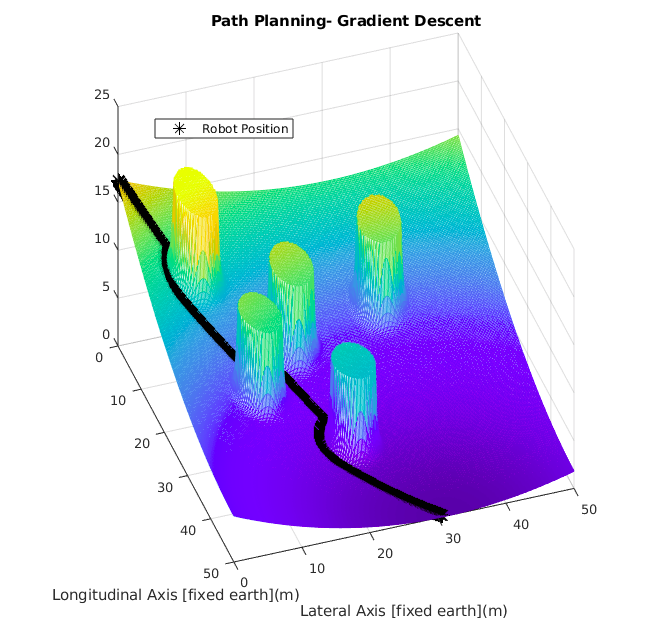
\includegraphics[scale=0.3]{img/scenario_1/apf.png}
    \caption{Scenario 1: Path Planning}
    \label{fig:scen_1_apf}
\end{figure}

Simulation is carried out using each of the 3 controllers, 
and their performances compared using the scaled error norm which is evaluated as an L2 norm of the lateral displacement tracking error divided by the number of time-steps. 

The PID controller is able to guide the system along the planned path best, yielding a scaled error norm of 0.0022 (Figure \ref{fig:scen_1_pid_lat}) 
albeit with a rather high peak control signal (front wheel steering angle) of about $-1.5rad \approx -85.94\deg$ which is not possible for typical wheel setups. 
The SIMO-based MPC performs a little better than the SISO-based MPC with error norms of 0.3647 (Figure \ref{fig:scen_1_mpc2_lat}) and 0.4714 (Figure \ref{fig:scen_1_mpc1_lat}) respectively. 
Both yielding control signals within the specified constraints of $\pm40\deg$. 

\begin{figure}
    \centering
    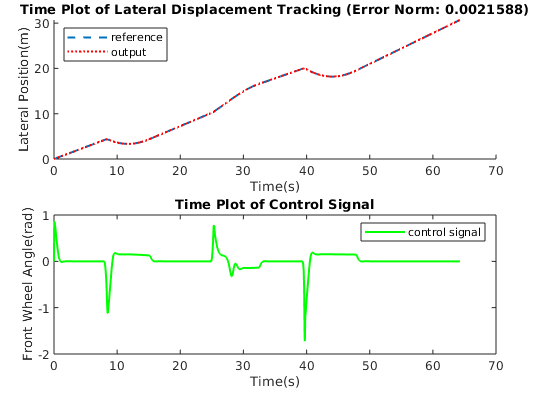
\includegraphics[scale=0.40]{img/scenario_1/pid-lat_tracking.png}
    \caption{Scenario 1: Lateral Displacement Tracking with PID Controller}
    \label{fig:scen_1_pid_lat}
\end{figure}

\begin{figure}
    \centering
    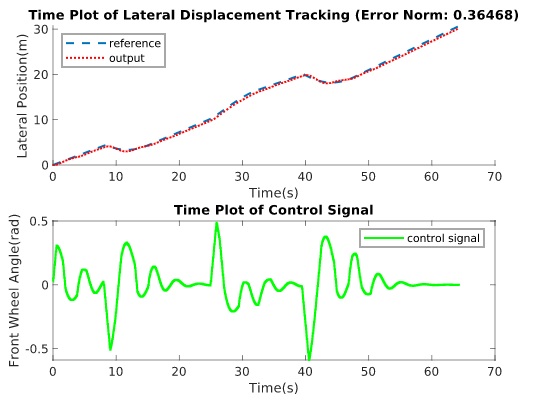
\includegraphics[scale=0.40]{img/scenario_1/mpc2-lat_tracking.png}
    \caption{Scenario 1: Lateral Displacement Tracking with SIMO MPC}
    \label{fig:scen_1_mpc2_lat}
\end{figure}

\begin{figure}
    \centering
    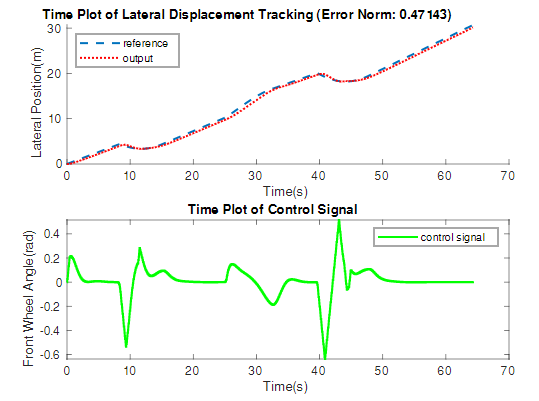
\includegraphics[scale=0.40]{img/scenario_1/mpc1-lat_tracking.png}
    \caption{Scenario 1: Lateral Displacement Tracking with SISO MPC}
    \label{fig:scen_1_mpc1_lat}
\end{figure}

Motion of the AMR through the simulation environment as controlled by the PID, SIMO-based MPC, and SISO-based MPC are shown in Figures \ref{fig:scen_1_pid_rob_mot}, \ref{fig:scen_1_mpc1_rob_mot}, and \ref{fig:scen_1_mpc2_rob_mot} respectively. 

\begin{figure}
    \centering
    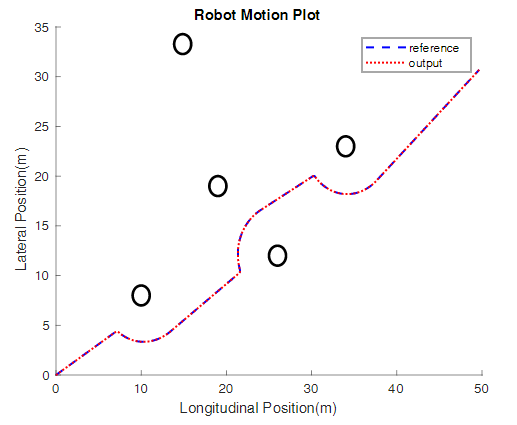
\includegraphics[scale=0.40]{img/scenario_1/pid-robot_motion.png}
    \caption{Scenario 1: AMR Motion in Simulation Environment for PID Controller}
    \label{fig:scen_1_pid_rob_mot}
\end{figure}

\begin{figure}
    \centering
    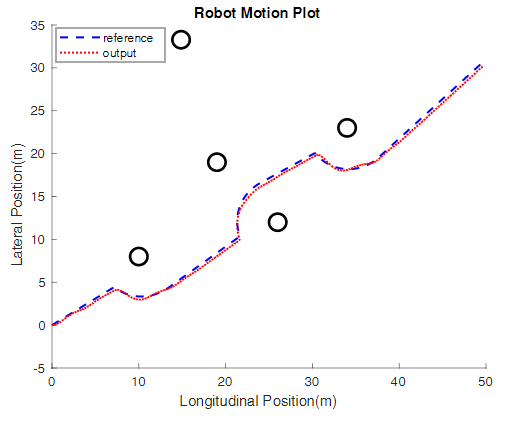
\includegraphics[scale=0.40]{img/scenario_1/mpc2-robot_motion.png}
    \caption{Scenario 1: AMR Motion in Simulation Environment for SIMO MPC}
    \label{fig:scen_1_mpc2_rob_mot}
\end{figure}

\begin{figure}
    \centering
    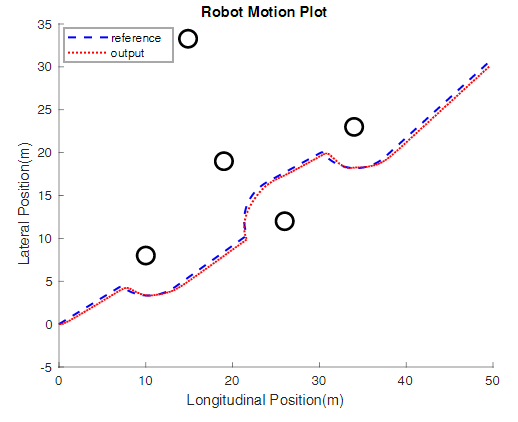
\includegraphics[scale=0.40]{img/scenario_1/mpc1-robot_motion.png}
    \caption{Scenario 1: AMR Motion in Simulation Environment for SISO MPC}
    \label{fig:scen_1_mpc1_rob_mot}
\end{figure}

The resulting yaw angles and yaw velocities from the PID controller, SIMO-based MPC, and SISO-based MPC are exhibited in Figures \ref{fig:scen_1_pid_yaw}, \ref{fig:scen_1_mpc2_yaw}, and \ref{fig:scen_1_mpc1_yaw} respectively. 

\begin{figure}
    \centering
    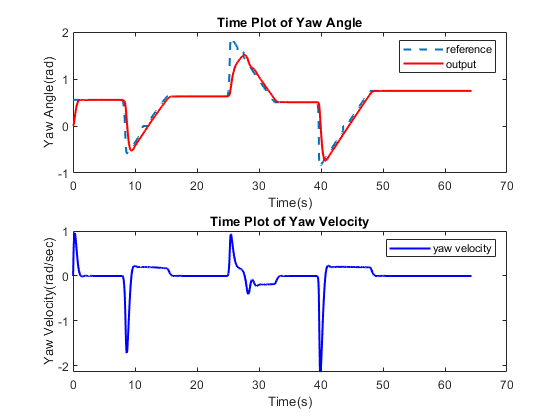
\includegraphics[scale=0.40]{img/scenario_1/pid-yaw.png}
    \caption{Scenario 1: Yaw Angle and Yaw Velocity resulting from PID Controller}
    \label{fig:scen_1_pid_yaw}
\end{figure}

\begin{figure}
    \centering
    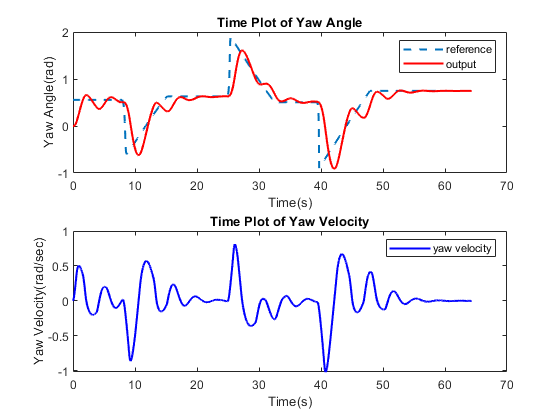
\includegraphics[scale=0.40]{img/scenario_1/mpc2-yaw.png}
    \caption{Scenario 1: Yaw Angle and Yaw Velocity resulting from SIMO MPC}
    \label{fig:scen_1_mpc2_yaw}
\end{figure}

\begin{figure}
    \centering
    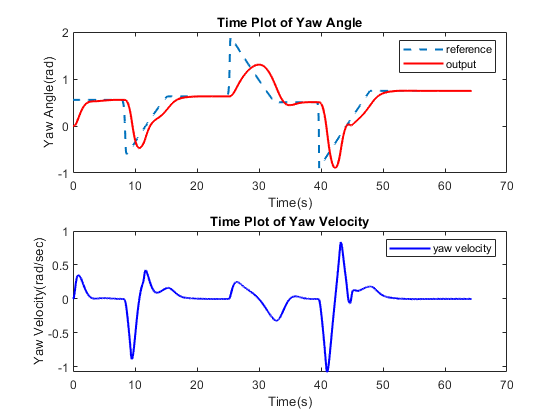
\includegraphics[scale=0.40]{img/scenario_1/mpc1-yaw.png}
    \caption{Scenario 1: Yaw Angle and Yaw Velocity resulting from SISO MPC}
    \label{fig:scen_1_mpc1_yaw}
\end{figure}

In conclusion, we can infer that the PID controller performed best, 
it would require some special wheel setup to pull off about $90\deg$ wheel angle. 
Further, the better performance of the SIMO-based MPC than the SISO-based MPC may be attributed to the extra yaw angle information available to the SIMO-based MPC. 


\subsection{Simulation Scenario 2}
As opposed to that of the simulation environment setup as described in Section 5.1.1,  
Figure \ref{fig:scen_2_apf} shows the universal potential field and the planned path. 

\begin{figure}
    \centering
    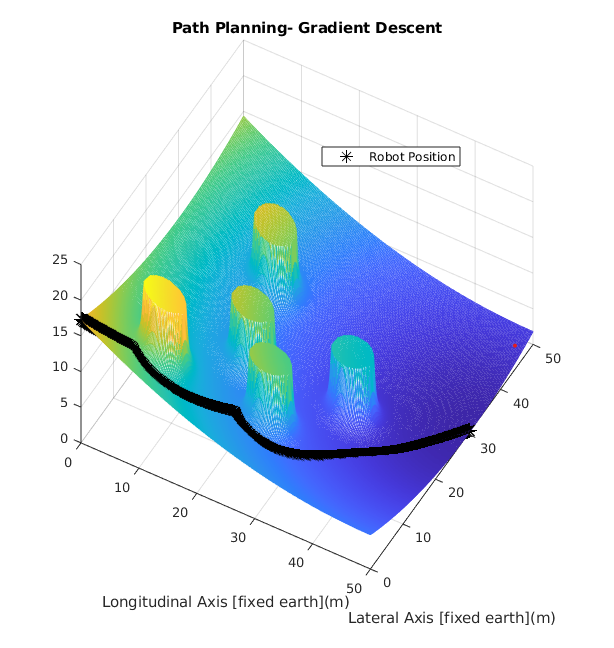
\includegraphics[scale=0.3]{img/scenario_2/apf.png}
    \caption{Scenario 2: Path Planning}
    \label{fig:scen_2_apf}
\end{figure}

Although the PID controller gives the lowest scaled error norm of 0.0044 (Figure \ref{fig:scen_2_pid_lat}), the control signal (front wheel steering angle) it produces is very unrealistic. 
The control signal rises up to about $-5.35rad \approx -306.53\deg$ at some point. 

\begin{figure}
    \centering
    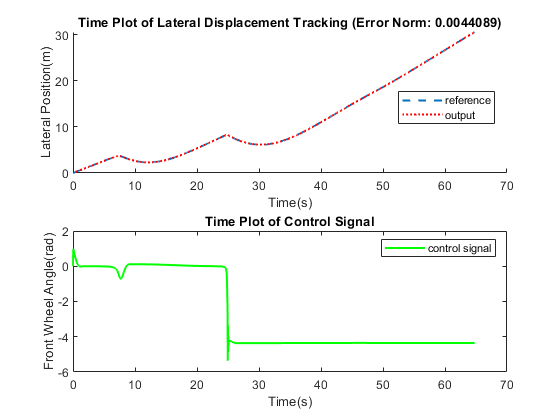
\includegraphics[scale=0.40]{img/scenario_2/pid-lateral_tracking.png}
    \caption{Scenario 2: Lateral Displacement Tracking with PID Controller}
    \label{fig:scen_2_pid_lat}
\end{figure}

The SIMO-based MPC is the controller of choice in this scenario, with a scaled error norm of 0.400 (Figure \ref{fig:scen_2_mpc2_lat}). 

\begin{figure}
    \centering
    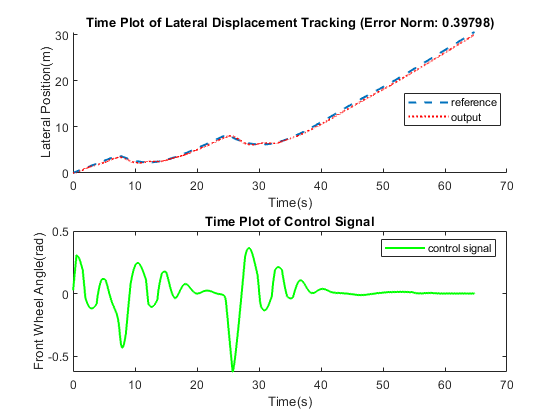
\includegraphics[scale=0.40]{img/scenario_2/mpc2-lateral_tracking.png}
    \caption{Scenario 2: Lateral Displacement Tracking with SIMO MPC}
    \label{fig:scen_2_mpc2_lat}
\end{figure}

The SISO-based MPC produced the largest scaled error norm of 0.4939 (Figure \ref{fig:scen_2_mpc1_lat}). 
Both yielding control signals within the specified constraints of $\pm40\deg$. 

\begin{figure}
    \centering
    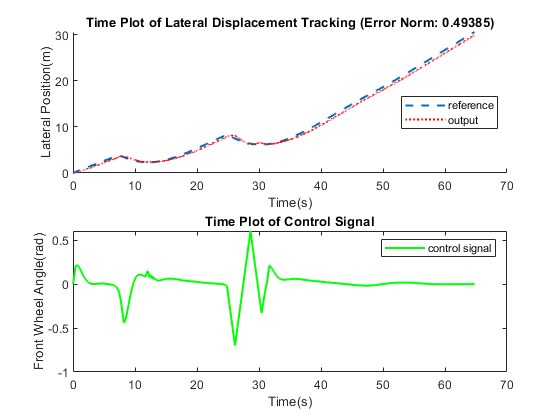
\includegraphics[scale=0.40]{img/scenario_2/mpc1-lateral_tracking.png}
    \caption{Scenario 2: Lateral Displacement Tracking with SISO MPC}
    \label{fig:scen_2_mpc1_lat}
\end{figure}

Motion of the AMR through the simulation environment as controlled by the PID, SIMO-based MPC, and SISO-based MPC are shown in Figures \ref{fig:scen_2_pid_rob_mot}, \ref{fig:scen_2_mpc1_rob_mot}, and \ref{fig:scen_2_mpc2_rob_mot} respectively. 

\begin{figure}
    \centering
    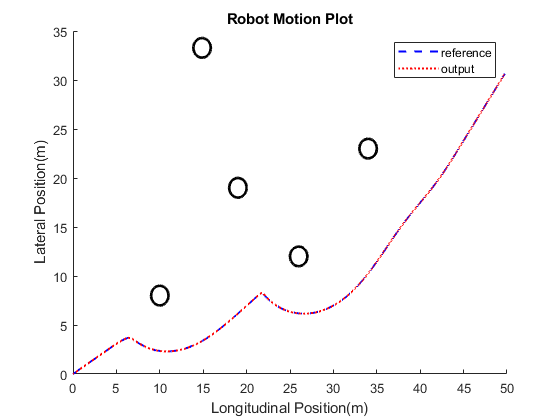
\includegraphics[scale=0.40]{img/scenario_2/pid-robot_motion.png}
    \caption{Scenario 2: AMR Motion in Simulation Environment for PID Controller}
    \label{fig:scen_2_pid_rob_mot}
\end{figure}

\begin{figure}
    \centering
    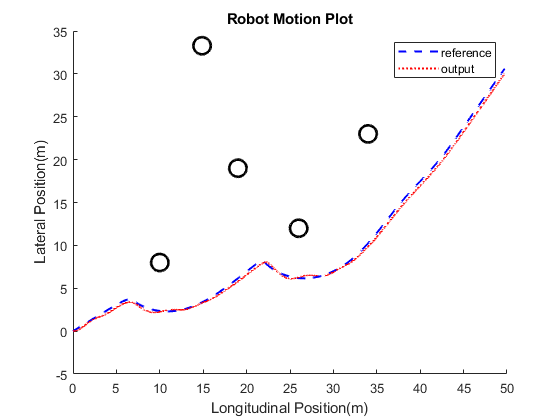
\includegraphics[scale=0.40]{img/scenario_2/mpc2-robot_motion.png}
    \caption{Scenario 2: AMR Motion in Simulation Environment for SIMO MPC}
    \label{fig:scen_2_mpc2_rob_mot}
\end{figure}

\begin{figure}
    \centering
    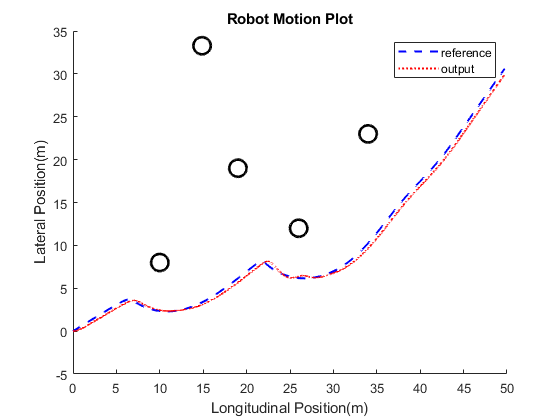
\includegraphics[scale=0.40]{img/scenario_2/mpc1-robot_motion.png}
    \caption{Scenario 2: AMR Motion in Simulation Environment for SISO MPC}
    \label{fig:scen_2_mpc1_rob_mot}
\end{figure}


In conclusion, we can infer that while the PID controller cannot be implemented in this scenario. 
Rather, the SIMO-based MPC should be used. 


\subsection{Simulation Scenario 3}
The simulation environment is setup as described in Section 5.1.1 however, an error is introduced such that the initial position of the AMR as seen by the path planning 
algorithm is $(0,0)$, while the initial position of the AMR in simulation is actually $(0,1)$. 
For this scenario, only the performance of the MPC controllers are evaluated. 
Figure \ref{fig:scen_1_apf} shows the universal potential field and the planned path which remains the same as from scenario 1. 

\begin{figure}
    \centering
    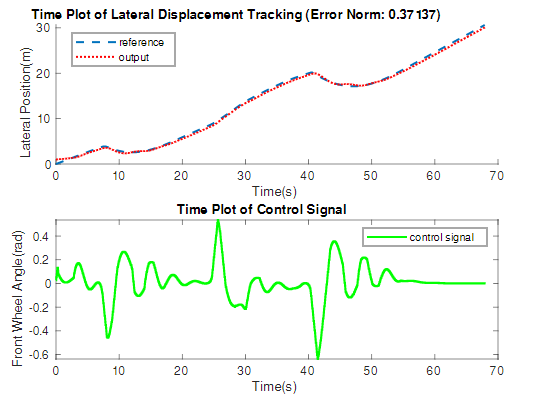
\includegraphics[scale=0.40]{img/scenario_3/mpc2-lat_tracking.png}
    \caption{Scenario 3: Lateral Displacement Tracking with SIMO MPC}
    \label{fig:scen_2_mpc2_lat}
\end{figure}

\begin{figure}
    \centering
    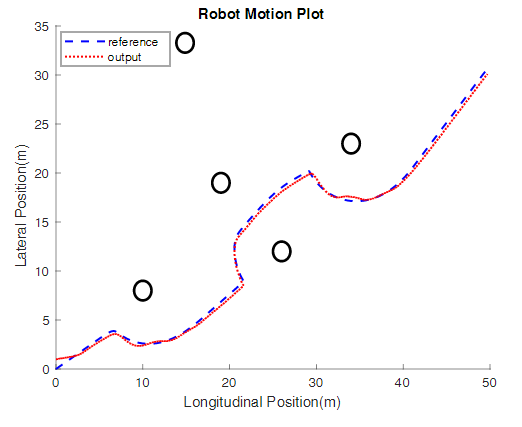
\includegraphics[scale=0.40]{img/scenario_3/mpc2-robot_motion.png}
    \caption{Scenario 3: AMR Motion in Simulation Environment for SIMO MPC}
    \label{fig:scen_2_mpc2_rob_mot}
\end{figure}

The SIMO-based MPC is able to overcome this initial error and guide the AMR onto the planned path as evident in Figures \ref{fig:scen_2_mpc2_lat} and \ref{fig:scen_2_mpc2_rob_mot}. 
However looking at Figure \ref{fig:scen_2_mpc1_lat_25} shows that the SISO-based MPC is unable to do so. 
Instead, lateral control of the AMR becomes unstable and as a result, the AMR starts going in circles as can be seen in Figure \ref{fig:scen_2_mpc1_rob_mot_25}. 
For this behavior to be visualized, the assumption of perfect longitudinal tracking is revoked. 

\begin{figure}
    \centering
    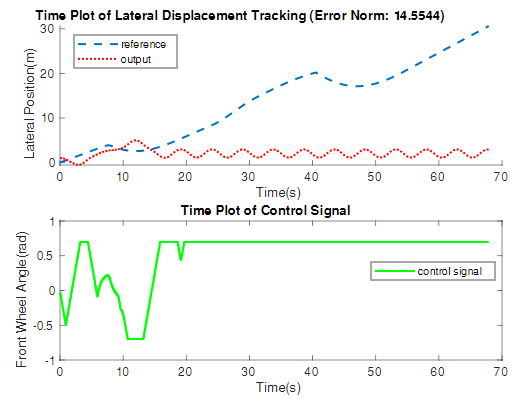
\includegraphics[scale=0.40]{img/scenario_3/mpc1_25-lat_tracking.png}
    \caption{Scenario 3: Lateral Displacement Tracking with SISO MPC}
    \label{fig:scen_2_mpc1_lat_25}
\end{figure}

\begin{figure}
    \centering
    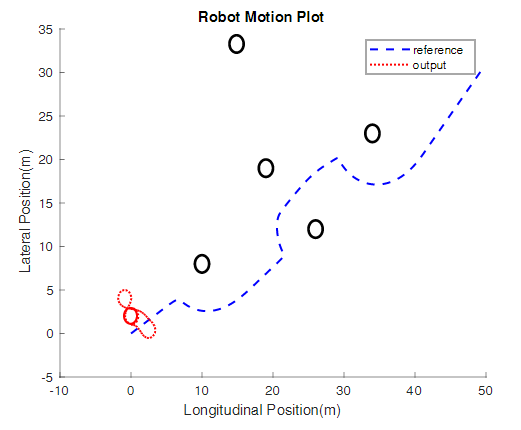
\includegraphics[scale=0.40]{img/scenario_3/mpc1_25-robot_motion.png}
    \caption{Scenario 3: AMR Motion in Simulation Environment for SISO MPC}
    \label{fig:scen_2_mpc1_rob_mot_25}
\end{figure}

The prediction horizon of the SISO-based MPC is increased from 25 time-steps to 35 time-steps to enable it predict the behavior of the AMR further in time. 
The results of simulation with this increase are displayed in Figures \ref{fig:scen_2_mpc1_lat_35} and \ref{fig:scen_2_mpc1_rob_mot_35} . 
With a prediction horizon of 35 time-steps, the SISO-based MPC is also able to overcome the initial error and guide the AMR onto the planned path. 

\begin{figure}[H]
    \centering
    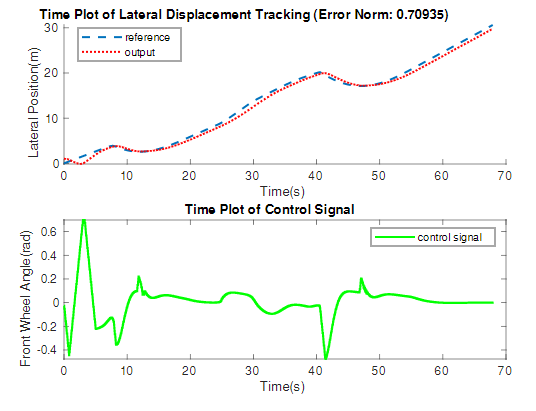
\includegraphics[scale=0.40]{img/scenario_3/mpc1_35-lat_tracking.png}
    \caption{Scenario 3: Lateral Displacement Tracking with SISO MPC with extended Prediction Horizon}
    \label{fig:scen_2_mpc1_lat_35}
\end{figure}

\begin{figure}[H]
    \centering
    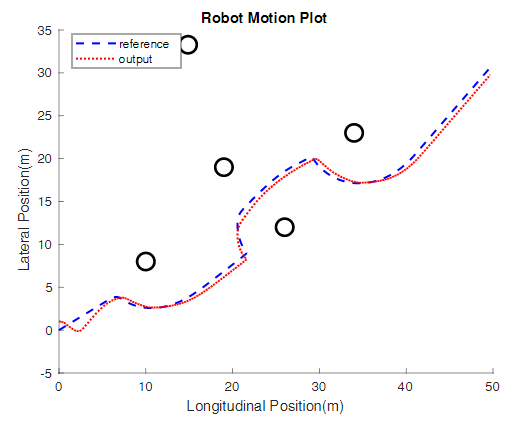
\includegraphics[scale=0.40]{img/scenario_3/mpc1_35-robot_motion.png}
    \caption{Scenario 3: AMR Motion in Simulation Environment for SISO MPC with extended Prediction Horizon}
    \label{fig:scen_2_mpc1_rob_mot_35}
\end{figure}


%===============================================================================================================%
% Conclusion
\section{Conclusion}
In an indoor environment with an accurate mapping and localization scheme, 
path planning and obstacle avoidance for Autonomous Mobile Robots moving at an average velocity can be successfully carried out using 
an Artificial Potential Field based approach and Model Predictive Control.

\bibliographystyle{plain}
\bibliography{references} 

\end{document}
